\section{Аберрации оптических систем. Аберрации, обусловленные широкими пучками лучей. Коррекция сферической и хроматической аберрации.}
\subsection{Аберрации оптических систем.}
	\Def{Аберрации оптических систем} (лат. aberratio - уклонение),
	погрешности изображений, даваемых оптическими системами.
	Проявляются в том, что оптические изображения в ряде случаев не
	вполне отчётливы, не точно соответствуют объекту или оказываются
	окрашенными.
Аберации делят на \textbf{\textit{монохроматические (геометрические)}} и \textbf{\textit{хроматические}}, среди геометрических выделяют
\begin{itemize}
	\item Сферическая аберрация
	\item Кома
	\item Астигматизм
	\item Дисторсия 
	\item Кривизна поля (поверхности) изображения
\end{itemize}
\subsubsection{Классификация геометрических аберраций}
Геометрические аберрации практически всегда являются учётом непараксиальности в ходе лучей. Произвольный луч в пространстве можно задать, указав прямоугольные координаты $y$, $z$, $\eta$ и $\zeta$ точек его пересечения с  предметной плоскостью (т.е. плоскостью, проходящей через изображаемую точку $P$ перпендикулярно к главной оптической оси) и плоскостью входного зрачка. После прохождения через оптическую систему луч пересечёт плоскость параксиального изображения в точке с координатами $y'$ и $z'$. Координаты самого параксиального изображения (\textit{параксиального фокуса}) -- $y_{0}'$, $z'_{0}$. Разности
\begin{align*}
\Delta y' &= y' - y'_{0} & \Delta z' &= z'- z'_{0}
\end{align*} 
примем за меру отступления от предельного случая параксиальной оптики.
Координаты $y'$  и  $z'$ будут функциями $y$, $z$, $\eta$ и $\zeta$:
\begin{align*}
y' &= f_{y}(y,z,\eta,\zeta) & z' &= f_{z}(y,z,\eta,\zeta)
\end{align*}
Линейные члены разложений $f_{y}$ и $f_{z}$ не зависят от $\eta$ и $\zeta$ и соответствуют параксиальной оптике, члены чётных степеней не войдут в эти разложения в силу осевой симметрии оптической задачи. Поэтому $\Delta y'$ и $\Delta z'$ будут определятся третьими членами разложения $f_{y}$ и $f_{z}$ (поэтому часто рассматриваемые дальше аберрации называются аберрациями третьего порядка).
 
Введём три вектора, перпендикулярных главной оптической оси системы:
\begin{align*}
\mathbf{r} &= y\mathbf{j} + z\mathbf{k} & \mathbf{r}' &= y'\mathbf{j} + z'\mathbf{k} & \bm{\sigma} &= \eta\mathbf{j} + \zeta\mathbf{k}
\end{align*}
Тогда вектор 
\begin{equation*}
\Delta \mathbf{r}' = \Delta y'\mathbf{j} + \Delta z'\mathbf{k}
\end{equation*}
может быть разложен по векторам $\mathbf{r}$ и $\bm{\sigma}$.
Причём в виду симметрии коэффициенты этих разложения могут зависеть только от <<инвариантов вращения>> $\bm{\sigma}^{2}$, $(\bm{\sigma}\mathbf{r})$ и $r^{2}$:
\begin{equation}
\label{series3}
\Delta \mathbf{r}' \approx \Big(A\bm{\sigma}^{2} + B(\bm{\sigma}\mathbf{r}) + C\mathbf{r}^{2}\Big)\bm{\sigma} + \Big(D\bm{\sigma}^{2} + E(\bm{\sigma}\mathbf{r}) + F\mathbf{r}^{2}\Big)\mathbf{r}
\end{equation}
В дальнейшем под $|\bm{\sigma}|$ понимается радиус входного зрачка. \textit{Аберрационной} кривой называют кривую, по которой плоскость параксиального изображения пересекает пучок лучей, проведённых из точки-объекта $P$ через окружность входного зрачка. Изображением вместо точки теперь окажется область, ограниченная аберрационной кривой.

Каждый из постоянных коэффициентов $A$, $B$, $C$, $D$, $E$ и $F$ в уравнении (\ref{series3}) определяется конфигурацией оптической системы и отвечает за конкретный тип аберрации. Аберрация определяемая членом $A\bm{\sigma}^{2}\bm{\sigma}$ называется \color{blue}{сферической}\normalcolor. Членам $B(\bm{\sigma}\mathbf{r})\bm{\sigma} + D\bm{\sigma}^{2}\mathbf{r}$ соответствует \color{blue}{кома}\normalcolor. Членам $C\mathbf{r}^{2}\bm{\sigma} + E(\bm{\sigma} r)\mathbf{r}$ -- \color{blue}{астигматизм косых лучей} \normalcolor и \color{blue}{искривление плоскости изображения}\normalcolor. Члену $F\mathbf{r}^{2}\mathbf{r}$  соответствует \color{blue}{дисторсия}\normalcolor.
\subsubsection{Сферическая аберрация}
\begin{figure}[H]
\begin{center}
\includegraphics[scale=0.36]{5_sferober.png}
\caption{Схема сферической аберрации, где
	$H$, $H'$ — положения главных плоскостей;
		$F'$  — задняя фокальная плоскость;
		$f'$  — заднее фокусное расстояние;
		$-\delta s'$  — продольная сферическая аберрация;
		$\delta g' = \Delta r'$  — поперечная сферическая аберрация.}
	\label{p1}
	\end{center}
	\end{figure}
	\Def{Сферическая аберрация} — аберрация оптических систем из-за несовпадения фокусов для лучей света, проходящих на разных расстояниях от оптической оси (см. рис.~\ref{p1}.).
ак как сферическая аберрация отвечает члену $A\bm{\sigma}^{2}\bm{\sigma}$, то если в системе есть только этот тип аберрации ($|B|,|C|,|D|,|E|,|F|\approx0\ll |A|$), то
\begin{equation*}
\Delta r'| = A\sigma^{3} = const
\end{equation*} 
 Значит аберрационной кривой является окружность (радиус которой пропорционален кубу входного зрачка), а изображение -- круглое пятнышко, ограниченное этой окружностью (см. рис.1).

\begin{wrapfigure}{r}{0.5\textwidth}
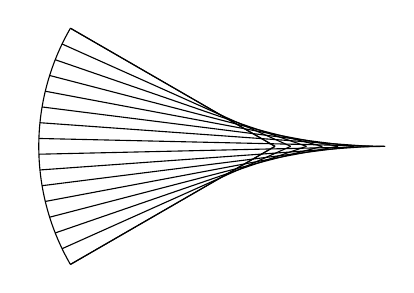
\begin{tikzpicture}
\draw (-2.598,-1.5) arc (210:150:3);
\draw (-2.598,1.5) -- (0,0);
\draw (-2.598,-1.5) -- (0,0);
\draw (-2.598,1.5) -- (0,0);
\draw (-2.598,-1.5) -- (0,0);
\draw (-2.704,1.3) -- (0.2,0);
\draw (-2.704,-1.3) -- (0.2,0);
\draw (-2.791,1.1) -- (0.4,0);
\draw (-2.791,-1.1) -- (0.4,0);
\draw (-2.862,0.9) -- (0.6,0);
\draw (-2.862,-0.9) -- (0.6,0);
\draw (-2.917,0.7) -- (0.8,0);
\draw (-2.917,-0.7) -- (0.8,0);
\draw (-2.958,0.5) -- (1.0,0);
\draw (-2.958,-0.5) -- (1.0,0);
\draw (-2.985,0.3) -- (1.2,0);
\draw (-2.985,-0.3) -- (1.2,0);
\draw (-2.998,0.1) -- (1.4,0);
\draw (-2.998,-0.1) -- (1.4,0);
\end{tikzpicture}
\caption{Каустика -- огибающая лучей от фронта}
\end{wrapfigure}
 В результате сферической аберрации цилиндрический пучок лучей, после преломления линзой (в пространстве изображений) получает вид не конуса, а некоторой воронкообразной фигуры, наружная поверхность которой, вблизи узкого места, называется каустической поверхностью. При этом изображение точки имеет вид диска с неоднородным распределением освещённости, а форма каустической кривой позволяет судить о характере распределения освещённости. В общем случае, фигура рассеяния, при наличии сферической аберрации, представляет собой систему концентрических окружностей с радиусами пропорциональными третьей степени координат на входном (или выходном) зрачке.

\begin{wrapfigure}{r}{0.55\textwidth}
\begin{tikzpicture}[>=latex']
\draw[black] (-2.598,-1.5) arc (210:150:3);
\draw[black] (-2.4,-1.5) arc (-30:30:3);
\draw[black] (-2.4,-1.5) -- (-2.598,-1.5); 
\draw[black] (-2.4,1.5) -- (-2.598,1.5);
\draw[black,->] (-4,-1.2) -- (-3,-1.2);
\draw[black] (-4,-1.2) -- (-2.75,-1.2);
\draw[black,->] (-4,1.2) -- (-3,1.2);
\draw[black] (-4,1.2) -- (-2.75,1.2);
\draw[red,->] (-2.75,1.2) -- (-2.22,1.15);
\draw[green,->] (-2.75,1.2) -- (-2.2,1.1);
\draw[blue,->] (-2.75,1.2) -- (-2.18,1.05);
\draw[red,->] (-2.75,-1.2) -- (-2.22,-1.15);
\draw[green,->] (-2.75,-1.2) -- (-2.2,-1.1);
\draw[blue,->] (-2.75,-1.2) -- (-2.18,-1.05);
\draw[red] (-2.22,1.15) -- (2,0);
\draw[green] (-2.2,1.1) -- (1.5,0);
\draw[blue] (-2.18,1.05) -- (1,0);
\draw[red] (-2.22,-1.15) -- (2,0);
\draw[green] (-2.2,-1.1) -- (1.5,0);
\draw[blue] (-2.18,-1.05) -- (1,0);
\draw[red,->] (-2.22,1.15) -- (-0.11,0.575);
\draw[green,->] (-2.2,1.1) -- (-0.35,0.55);
\draw[blue,->] (-2.18,1.05) -- (-0.59,0.525);
\draw[red,->] (-2.22,-1.15) -- (-0.11,-0.575);
\draw[green,->] (-2.2,-1.1) -- (-0.35,-0.55);
\draw[blue,->] (-2.18,-1.05) -- (-0.59,-0.525);
\draw[gray,dashdotted] (-4,0)--(2.5,0);
\end{tikzpicture}
\caption{Пример хроматической аберрации.}
\label{p3}
\end{wrapfigure} 

Сферическая аберрация линзы (системы линз) объясняется тем, что её преломляющие поверхности встречают отдельные лучи сколько-нибудь широкого пучка под различными углами. Вследствие чего, более удалённые от оптической оси лучи преломляются сильнее, нежели нулевые лучи, и образуют свои точки схода удалённые от фокальной плоскости.
\subsubsection{Хроматическая аберрация}
Если используется белый свет, то в изображении возникают дополнительные аберрации. Это связано с тем, что показатель преломления зависит от длины волны (дисперсия света). Поэтому оптическая система даёт не одно, а множество монохроматических изображений, отличающихся друг от друга по величине и положению. Результирующее же изображение, получающееся от наложения таких монохроматических изображений, оказывается нерезким и с окрашенными краями. Это явление и называется \textit{хроматической аберрацией} (например рис.~\ref{p3}).
\subsection{Коррекция сферической и хроматической аберрации.}
И сферическая и хроматическая аберрации могут быть с той или иной мерой точности откорректированы путём комбинации линз (например, рис.~\ref{p4gl}).
\begin{figure}[H]
	\begin{center}
	\subfigure{\label{p40}}
	\begin{tikzpicture}[>=latex']
	\draw[black] (-2.598,-1.5) arc (210:150:3);
	\draw[black] (-2.4,-1.5) arc (-30:30:3);
	\draw[black] (-2.4,-1.5) -- (-2.598,-1.5); 
	\draw[black] (-2.4,1.5) -- (-2.598,1.5);
	\draw[black,->] (-4,-1.2) -- (-3,-1.2);
	\draw[black] (-4,-1.2) -- (-2.75,-1.2);
	\draw[black,->] (-4,1.2) -- (-3,1.2);
	\draw[black] (-4,1.2) -- (-2.75,1.2);
	\draw[red,->] (-2.75,1.2) -- (-2.22,1.15);
	\draw[green,->] (-2.75,1.2) -- (-2.2,1.1);
	\draw[blue,->] (-2.75,1.2) -- (-2.18,1.05);
	\draw[red,->] (-2.75,-1.2) -- (-2.22,-1.15);
	\draw[green,->] (-2.75,-1.2) -- (-2.2,-1.1);
	\draw[blue,->] (-2.75,-1.2) -- (-2.18,-1.05);
	\draw[red] (-2.22,1.15) -- (2,0);
	\draw[green] (-2.2,1.1) -- (1.5,0);
	\draw[blue] (-2.18,1.05) -- (1,0);
	\draw[red] (-2.22,-1.15) -- (2,0);
	\draw[green] (-2.2,-1.1) -- (1.5,0);
	\draw[blue] (-2.18,-1.05) -- (1,0);
	\draw[red,->] (-2.22,1.15) -- (-0.11,0.575);
	\draw[green,->] (-2.2,1.1) -- (-0.35,0.55);
	\draw[blue,->] (-2.18,1.05) -- (-0.59,0.525);
	\draw[red,->] (-2.22,-1.15) -- (-0.11,-0.575);
	\draw[green,->] (-2.2,-1.1) -- (-0.35,-0.55);
	\draw[blue,->] (-2.18,-1.05) -- (-0.59,-0.525);
	\draw[gray,dashdotted] (-4,0)--(2.5,0);
	\end{tikzpicture}
	\subfigure{\label{p4}}
	\begin{tikzpicture}[>=latex']
	\draw[black] (-2.598,-1.5) arc (210:150:3);
	\draw[black,thick] (-2.4,-1.5) arc (-30:30:3);
	\draw[black] (-2.4,-1.5) -- (-2.598,-1.5); 
	\draw[black] (-2.4,1.5) -- (-2.598,1.5);
	\draw[black,->] (-4,-1.2) -- (-3,-1.2);
	\draw[black] (-4,-1.2) -- (-2.75,-1.2);
	\draw[black,->] (-4,1.2) -- (-3,1.2);
	\draw[black] (-4,1.2) -- (-2.75,1.2);
	\draw[red,->] (-2.75,1.2) -- (-2.22,1.15);
	\draw[green,->] (-2.75,1.2) -- (-2.2,1.1);
	\draw[blue,->] (-2.75,1.2) -- (-2.18,1.05);
	\draw[red,->] (-2.75,-1.2) -- (-2.22,-1.15);
	\draw[green,->] (-2.75,-1.2) -- (-2.2,-1.1);
	\draw[blue,->] (-2.75,-1.2) -- (-2.18,-1.05);
	\draw[black] (-2.4,1.5) -- (-1.6,1.5) -- (-1.6,-1.5) -- (-2.4,-1.5);
	\draw[gray,dashdotted] (-4,0)--(2.5,0);
	%
	\draw[red,->] (-2.22,1.15) -- (-1.6,1.075);
	\draw[green,->] (-2.2,1.1) -- (-1.6,1.05);
	\draw[blue,->] (-2.18,1.05) -- (-1.6,1.03);
	\draw[red,->] (-2.22,-1.15) -- (-1.6,-1.075);
	\draw[green,->] (-2.2,-1.1) -- (-1.6,-1.05);
	\draw[blue,->] (-2.18,-1.05) -- (-1.6,-1.03);
	%
	\draw[red] (-1.6,1.075) -- (2.5,0);
	\draw[green] (-1.6,1.05) -- (2.3,0);
	\draw[blue] (-1.6,1.03) -- (2.1,0);
	\draw[red] (-1.6,-1.075) -- (2.5,0);
	\draw[green] (-1.6,-1.05) -- (2.3,0);
	\draw[blue] (-1.6,-1.03) -- (2.1,0);
	\draw[red,->] (-1.6,1.075) -- (0.45,0.5375);
	\draw[green,->] (-1.6,1.05) -- (0.35,0.525);
	\draw[blue,->] (-1.6,1.03) -- (0.25,0.515);
	\draw[red,->] (-1.6,-1.075) -- (0.45,-0.5375);
	\draw[green,->] (-1.6,-1.05) -- (0.35,-0.525);
	\draw[blue,->] (-1.6,-1.03) -- (0.25,-0.515);
	\end{tikzpicture}
	\end{center}
	\caption{Пример коррекции хроматической аберрации на собирающеё линзе при помощи рассеивающей линзы.}
	\label{p4gl}
\end{figure} 